\documentclass[../cours_2de.tex]{subfiles}
\begin{document}
\setcounter{chapter}{21}
\chapter{Probabilités conditionnelles et arbres}
\label{sec:ch22}
\begin{objectif}
Comprendre le changement d'univers lorsqu'une information est connue ; lire un arbre pondéré ; distinguer les deux sens d'un conditionnement.
\end{objectif}
\section{Changer la population de référence}
\begin{definition}
Si $P(A)>0$, la probabilité de $B$ sachant $A$ est
\[
P_A(B)=\frac{P(A\cap B)}{P(A)}.
\]
On rencontre aussi la notation $P(B\mid A)$.
\end{definition}
On conserve les issues de $A$ et on renormalise leurs probabilités pour que leur somme redevienne $1$.
En tirant un individu avec équiprobabilité dans une population finie,
$P_A(B)=\operatorname{Card}(A\cap B)/\operatorname{Card}(A)$ :
c'est la fréquence conditionnelle du chapitre 20.
\begin{exemple}
Sur un dé équilibré, sachant que le résultat est pair, la probabilité d'obtenir au moins $4$ vaut $2/3$ : les issues admissibles sont $2,4,6$, et deux conviennent.
Sans cette information, la probabilité serait $3/6=1/2$.
\end{exemple}
\begin{attention}
On ne définit pas $P_A(B)$ par ce quotient lorsque $P(A)=0$.
En général $P_A(B)\ne P_B(A)$ : les dénominateurs ne sont pas les mêmes.
\end{attention}
\section{Pourquoi multiplier le long d'un chemin ?}
\begin{propriete}
Pour $P(A)>0$, $P(A\cap B)=P(A)P_A(B)$.
Les branches issues d'un même nœud somment à $1$ :
$P_A(B)+P_A(\overline B)=1$.
\end{propriete}
\begin{demonstration}
La première formule vient de la définition, multipliée par $P(A)$.
Les événements $A\cap B$ et $A\cap\overline B$ partitionnent $A$.
Leurs probabilités somment à $P(A)$ ; diviser par cette valeur donne la deuxième formule.
\end{demonstration}
Un arbre pondéré inscrit les probabilités initiales au premier niveau, puis des probabilités conditionnelles aux niveaux suivants.
Le produit d'un chemin représente une intersection. Des feuilles distinctes décrivent des événements disjoints : leurs probabilités peuvent être additionnées.
\begin{exemple}[Deux tirages sans remise]
Avec trois boules rouges et deux bleues, la branche du premier rouge vaut $3/5$.
Après ce rouge, il reste deux rouges parmi quatre boules : la branche du second rouge vaut $2/4$.
Le chemin rouge--rouge vaut $(3/5)(2/4)=3/10$.
La branche du second rouge après un premier bleu vaut au contraire $3/4$.
\end{exemple}
\section{Inverser un conditionnement : test fictif}
On considère un modèle purement pédagogique de dépistage : $1\,\%$ d'une population est concerné par une condition $M$.
Le test est positif pour $90\,\%$ des personnes concernées (sensibilité) et négatif pour $95\,\%$ des autres (spécificité).
Ces nombres sont inventés ; ils ne décrivent aucun test réel.
\begin{center}
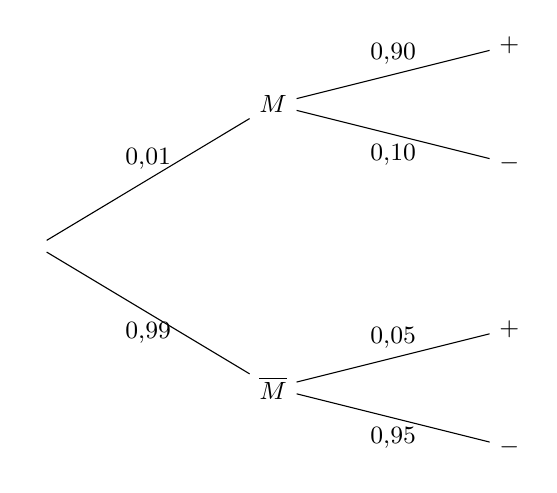
\begin{tikzpicture}[grow=right,level distance=3cm,
level 1/.style={sibling distance=3.6cm},
level 2/.style={sibling distance=1.5cm},
every node/.style={font=\small}]
\node {}
child {node {$\overline M$}
child {node {$-$} edge from parent node[below] {$0{,}95$}}
child {node {$+$} edge from parent node[above] {$0{,}05$}}
edge from parent node[below] {$0{,}99$}}
child {node {$M$}
child {node {$-$} edge from parent node[below] {$0{,}10$}}
child {node {$+$} edge from parent node[above] {$0{,}90$}}
edge from parent node[above] {$0{,}01$}};
\end{tikzpicture}
\end{center}
Sur une population théorique de $10000$ individus reproduisant ces proportions :
\[
\begin{array}{c|rr|r}
 &+&-&\text{total}\\\hline
M&90&10&100\\
\overline M&495&9405&9900\\\hline
\text{total}&585&9415&10000
\end{array}
\]
Les faux positifs sont les $495$ individus de $\overline M\cap+$ ; les faux négatifs les $10$ individus de $M\cap-$.
Ainsi $P_M(+)=90/100=0{,}90$, mais
$P_+(M)=90/585=2/13\simeq15{,}38\,\%$.
Une bonne sensibilité ne suffit donc pas à lire la probabilité inverse ; la fréquence de la condition dans la population compte aussi.
\section{Distinguer indépendance et incompatibilité}
\approfondissement Deux événements sont indépendants si $P(A\cap B)=P(A)P(B)$.
Lorsque $P(A)>0$, cela équivaut à $P_A(B)=P(B)$ : savoir $A$ ne modifie pas la probabilité de $B$.
Deux événements incompatibles ont une intersection vide. S'ils ont chacun une probabilité positive, ils ne sont pas indépendants, puisque $0\ne P(A)P(B)$.
Pour des tirages avec remise et mélange identique, l'indépendance peut être une hypothèse du modèle. Sans remise, elle n'est généralement pas vérifiée.
\begin{finchapitre}
\section{La formule générale, en approfondissement}
Le programme demande de comprendre et d'exploiter les arbres, mais la formule abstraite des probabilités totales n'est pas un attendu de seconde.
\approfondissement Si $A_1,\ldots,A_k$ forment une partition de l'univers et ont des probabilités positives, alors
\[
P(B)=\sum_{i=1}^k P(A_i)P_{A_i}(B).
\]
En effet, les $A_i\cap B$ sont disjoints et leur réunion vaut $B$ ; on utilise l'additivité puis la formule du chemin.
Si $P(B)>0$, la définition donne ensuite
$P_B(A_j)=P(A_j)P_{A_j}(B)/P(B)$.
Il s'agit de l'inversion du conditionnement, souvent appelée formule de Bayes.
\utilite{Le conditionnement rend explicite l'information disponible. Il permet de comprendre les tableaux, les arbres et les erreurs d'interprétation des tests.}
\begin{retenir}
À chaque probabilité, nommer la population de référence. Une branche après un événement décrit une conditionnelle ; une feuille décrit une intersection.
\end{retenir}
\end{finchapitre}
\end{document}
